\beginsong{Schilf}[
    wuw={tejo (Walter Scherf), Musik aus Schweden}, 
    pfii={61}, 
    pfiii={48}, 
    bo={272}, 
    kssiv={37}, 
    siru={203}, 
    index={Schilf bleicht die langen welkenden Haare},
]

\beginverse
\endverse
\centering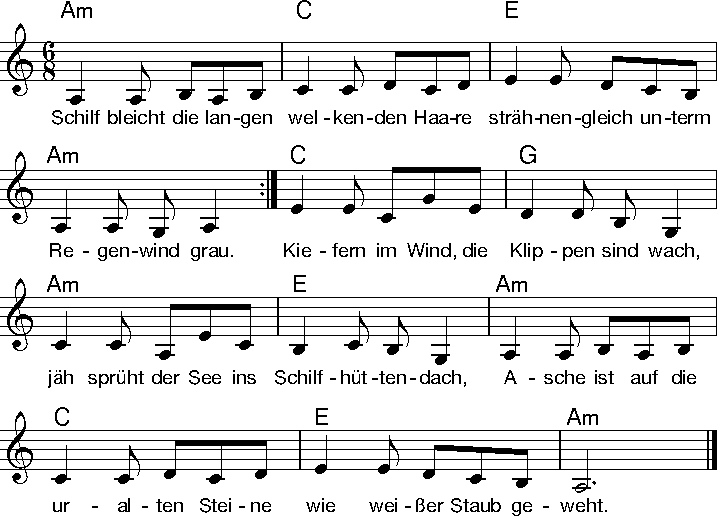
\includegraphics[width=1\textwidth]{Noten/Lied080.pdf}	

\beginverse
\[Am]Feuer ist in den \[C]dämmernden Stunden
\[E]lange erloschen, \[Am]Tag wird es schon.
\[Am]Graugänse sind am \[C]Morgen gekommen, 
\[E]welk auf der Schwelle \[Am]schläft roter Mohn.
\endverse
 
\beginchorus
\[C]Kiefern im Wind, die \[G]Klippen sind wach,
\[Am]jäh sprüht der See ins \[E]Schilfhüttendach.
\[Am]Asche ist auf die \[C]uralten Steine
\[E]wie weißer Staub ge\[Am]weht.
\endchorus

\beginverse
^Weht aus den Fugen ^weit in die Ödmark,
^frierend macht mich das ^Sturmbrausen taub.
^Schläft noch und träumt von ^Felsen und Birken,
^legt euch im Mantel ^unter das Laub.
\endverse

\printchorus

\beginverse
^Ach diese letzten ^Tage und Stunden,
^morgen ist unsre ^Fahrt schon vorbei.
^Weit ist die alte ^Tür aufgesprungen,
^strandhell erschallt der ^Herbstmöwe Schrei.
\endverse

\printchorus

\endsong
